\documentclass[10pt]{beamer} % aspect ratio 4:3, 128 mm by 96 mm

%\documentclass[10pt,aspectratio=169]{beamer} % aspect ratio 16:9

%\graphicspath{{../../figures/}}

\graphicspath{{figs/}{../../figures/}{../../../reports/figures/png/}}

%\includeonlyframes{frame1,frame2,frame3,frame4,frame5,frame6,frame7,frame8,frame9}

%\includeonlyframes{frame10,frame11,frame12,frame13}

%\includeonlyframes{frame14,frame15,frame16,frame17,frame18,frame19,frame20,frame21}

%\includeonlyframes{frame22,frame23,frame24,frame25,frame26}

%\includeonlyframes{frame27,frame28}

%%%%%%%%%%%%%%%%%%%%%%%%%%%%%%%%%%%%%%%%%%%%%%%%%%

% Packages

%%%%%%%%%%%%%%%%%%%%%%%%%%%%%%%%%%%%%%%%%%%%%%%%%%

\usepackage{appendixnumberbeamer}

\usepackage{booktabs}

\usepackage{pgfplots}

\usepackage{xspace}

\usepackage{amsmath}

\usepackage{multirow}

\usepackage{totcount}

\usepackage{tikz}

%\usepackage{comment}

%\usetikzlibrary{external} % speedup compilation

%\tikzexternalize % activate!

%\usetikzlibrary{shapes,arrows}  


%\usepackage{bibentry}

%\nobibliography*

\usepackage{caption}%

\captionsetup[figure]{labelformat=empty}%

%%%%%%%%%%%%%%%%%%%%%%%%%%%%%%%%%%%%%%%%%%%%%%%%%%

% Metropolis theme custom modification file

%%%%%%%%%%%%%%%%%%%%%%%%%%%%%%%%%%%%%%%%%%%%%%%%%%
% Metropolis theme custom modification file
%%%%%%%%%%%%%%%%%%%%%%%%%%%%%%%%%%%%%%%%%%%%%%%%%%
% Metropolis theme custom colors
%%%%%%%%%%%%%%%%%%%%%%%%%%%%%%%%%%%%%%%%%%%%%%%%%%
\usetheme[progressbar=foot]{metropolis}
\useoutertheme{metropolis}
\useinnertheme{metropolis}
\usefonttheme{metropolis}
\setbeamercolor{background canvas}{bg=white}

%\usecolortheme{spruce}

\definecolor{myblue}{rgb}{0.19,0.55,0.91}
\definecolor{mediumblue}{rgb}{0,0,205}
\definecolor{darkblue}{rgb}{0,0,139}
\definecolor{Dodgerblue}{HTML}{1E90FF}
\definecolor{Navy}{HTML}{000080} % {rgb}{0,0,128}
\definecolor{Aliceblue}{HTML}{F0F8FF}
\definecolor{Lightskyblue}{HTML}{87CEFA}
\definecolor{logoblue}{RGB}{1,67,140}
\definecolor{Purple}{HTML}{911146}
\definecolor{Orange}{HTML}{CF4A30}

\setbeamercolor{progress bar}{bg=Lightskyblue}
\setbeamercolor{progress bar}{ fg=logoblue} 
\setbeamercolor{frametitle}{bg=logoblue}
\setbeamercolor{title separator}{fg=logoblue}
\setbeamercolor{block title}{bg=Lightskyblue!30,fg=black}
\setbeamercolor{block body}{bg=Lightskyblue!15,fg=black}
\setbeamercolor{alerted text}{fg=Purple}
%%%%%%%%%%%%%%%%%%%%%%%%%%%%%%%%%%%%%%%%%%%%%%%%%%
%  Theme modifications
%%%%%%%%%%%%%%%%%%%%%%%%%%%%%%%%%%%%%%%%%%%%%%%%%%
% modify progress bar linewidth
\makeatletter
\setlength{\metropolis@progressinheadfoot@linewidth}{2pt} 
\setlength{\metropolis@titleseparator@linewidth}{1pt}
\setlength{\metropolis@progressonsectionpage@linewidth}{1pt}

\setbeamertemplate{progress bar in section page}{
	\setlength{\metropolis@progressonsectionpage}{%
		\textwidth * \ratio{\thesection pt}{\totvalue{totalsection} pt}%
	}%
	\begin{tikzpicture}
	\fill[bg] (0,0) rectangle (\textwidth, \metropolis@progressonsectionpage@linewidth);
	\fill[fg] (0,0) rectangle (\metropolis@progressonsectionpage, \metropolis@progressonsectionpage@linewidth);
	\end{tikzpicture}%
}
\makeatother
\newcounter{totalsection}
\regtotcounter{totalsection}

\AtBeginDocument{%
	\pretocmd{\section}{\refstepcounter{totalsection}}{\typeout{Yes, prepending was successful}}{\typeout{No, prepending was not successful}}%
}%
%%%%%%%%%%%%%%%%%%%%%%%%%%%%%%%%%%%%%%%%%%%%%%%%%%
%  Bibliography mods
%%%%%%%%%%%%%%%%%%%%%%%%%%%%%%%%%%%%%%%%%%%%%%%%%%
\setbeamertemplate{bibliography item}{\insertbiblabel} %% Remove book symbol from references and add number in square brackets
% kill the abominable icon (without number)
%\setbeamertemplate{bibliography item}{}
%\makeatletter
%\renewcommand\@biblabel[1]{#1.} % number only
%\makeatother
% remove line breaks in bibliography
\setbeamertemplate{bibliography entry title}{}
\setbeamertemplate{bibliography entry location}{}
%%%%%%%%%%%%%%%%%%%%%%%%%%%%%%%%%%%%%%%%%%%%%%%%%%
%  Bibliography custom commands
%%%%%%%%%%%%%%%%%%%%%%%%%%%%%%%%%%%%%%%%%%%%%%%%%%
\newcommand{\bibliotitlestyle}[1]{\textbf{#1}\par}

\newif\ifinbiblio
\newcounter{bibkey}
\newenvironment{biblio}[2][long]{%
    %\setbeamertemplate{bibliography item}{\insertbiblabel}
    \setbeamertemplate{bibliography item}{}% without numbers
	\setbeamerfont{bibliography item}{size=\footnotesize}
	\setbeamerfont{bibliography entry author}{size=\footnotesize}
	\setbeamerfont{bibliography entry title}{size=\footnotesize}
	\setbeamerfont{bibliography entry location}{size=\footnotesize}
	\setbeamerfont{bibliography entry note}{size=\footnotesize}
	\ifx!#2!\else%
	\bibliotitlestyle{#2}%
	\fi%
	\begin{thebibliography}{}%
		\inbibliotrue%
		\setbeamertemplate{bibliography entry title}[#1]%
	}{%
		\inbibliofalse%
		\setbeamertemplate{bibliography item}{}%
	\end{thebibliography}%
}

\newcommand{\biblioref}[5][short]{
	\setbeamertemplate{bibliography entry title}[#1]
	\stepcounter{bibkey}%
	\ifinbiblio%
	\bibitem{\thebibkey}%
	#2
	\newblock #4
	\ifx!#5!\else\newblock {\em #5}, #3 \fi%
	\else%
	\begin{biblio}{}
		\bibitem{\thebibkey}
		#2
		\newblock #4
		\ifx!#5!\else\newblock {\em #5}, #3\fi
	\end{biblio}
	\fi
}
%
%\newbibmacro*{hypercite}{%
%	\renewcommand{\@makefntext}[1]{\noindent\normalfont##1}%
%	\footnotetext{%
%		\blxmkbibnote{foot}{%
%			\printtext[labelnumberwidth]{%
%				\printfield{prefixnumber}%
%				\printfield{labelnumber}}%
%			\addspace
%			\fullcite{\thefield{entrykey}}}}}
%
%\DeclareCiteCommand{\hypercite}%
%{\usebibmacro{cite:init}}
%{\usebibmacro{hypercite}}
%{}
%{\usebibmacro{cite:dump}}
%
%% Redefine the \footfullcite command to use the reference number
%\renewcommand{\footfullcite}[1]{\cite{#1}\hypercite{#1}}

%%%%%%%%%%%%%%%%%%%%%%%%%%%%%%%%%%%%%%%%%%%%%%%%%%

% Custom commands

%%%%%%%%%%%%%%%%%%%%%%%%%%%%%%%%%%%%%%%%%%%%%%%%%%

% matrix command 

\newcommand{\matr}[1]{\mathbf{#1}} % bold upright (Elsevier, Springer)

%\newcommand{\matr}[1]{#1}          % pure math version

%\newcommand{\matr}[1]{\bm{#1}}     % ISO complying version

% vector command 

\newcommand{\vect}[1]{\mathbf{#1}} % bold upright (Elsevier, Springer)

% bold symbol

\newcommand{\bs}[1]{\boldsymbol{#1}}

% derivative upright command

\DeclareRobustCommand*{\drv}{\mathop{}\!\mathrm{d}}

\newcommand{\ud}{\mathrm{d}}

% 

\newcommand{\themename}{\textbf{\textsc{metropolis}}\xspace}


%%%%%%%%%%%%%%%%%%%%%%%%%%%%%%%%%%%%%%%%%%%%%%%%%%

%  Title page options

%%%%%%%%%%%%%%%%%%%%%%%%%%%%%%%%%%%%%%%%%%%%%%%%%%

% \date{\today}

\date{}

%%%%%%%%%%%%%%%%%%%%%%%%%%%%%%%%%%%%%%%%%%%%%%%%%%

% option 1

%%%%%%%%%%%%%%%%%%%%%%%%%%%%%%%%%%%%%%%%%%%%%%%%%%

\title{Modelling of sandwich plates and piezoelectric transducers to identify the severity of mechanical damage}

\author{\textbf{Piotr Fiborek, M.Sc. Eng.}, \\
	supervisor: Pawel Kudela, D.Sc. Ph.D. Eng.}

% logo align to Institute 

\institute{Institute of Fluid Flow Machinery\\Polish Academy of Sciences \\ \vspace{-1.5cm}\flushright 
\includegraphics[width=4cm]{logo_eng_40mm.eps}}

%%%%%%%%%%%%%%%%%%%%%%%%%%%%%%%%%%%%%%%%%%%%%%%%%%


%%%%%%%%%%%%%%%%%%%%%%%%%%%%%%%%%%%%%%%%%%%%%%%%%%

\begin{document}

	%%%%%%%%%%%%%%%%%%%%%%%%%%%%%%%%%%%%%%%%%%%%%%%%%%

	\maketitle

	%%%%%%%%%%%%%%%%%%%%%%%%%%%%%%%%%%%%%%%%%%%%%%%%%%

	% SLIDES

	%%%%%%%%%%%%%%%%%%%%%%%%%%%%%%%%%%%%%%%%%%%%%%%%%%

	\begin{frame}[label=frame1]{Table of contents \label{frameone}}

		\setbeamertemplate{section in toc}[sections numbered]

		\tableofcontents[hideallsubsections]

	\end{frame}

	%%%%%%%%%%%%%%%%%%%%%%%%%%%%%%%%%%%%%%%%%%%%%%%%%%

	\section{Introduction}

	%%%%%%%%%%%%%%%%%%%%%%%%%%%%%%%%%%%%%%%%%%%%%%%%%%

	
	\begin{frame}[label=frame2]{Sandwich Composite Properties}

		\begin{columns}[T]

			\column{0.5\textwidth}

			\begin{block}{Sandwich Composite Structures}

				\begin{itemize}

					\item Multi-layered structure composed of a mid-core and thin skins

					\item High strength-to-density ratio

					\item High acoustic or fire insulation properties

				\end{itemize}

			\end{block}

			\column{0.5\textwidth}

			\begin{figure}

				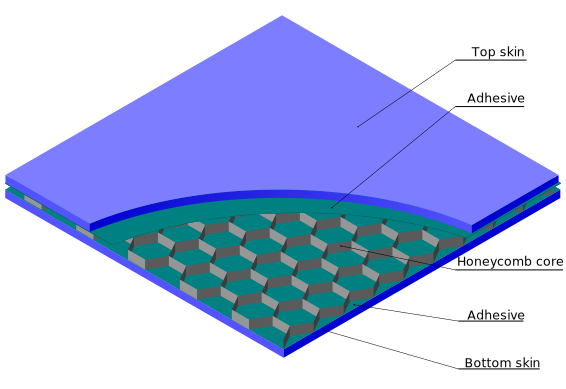
\includegraphics[width=0.9\textwidth]{honeycomb_plate.png}

				\caption{Honeycomb Sandwich Panel (HSP)}

			\end{figure}

		\end{columns}

	\end{frame}

	\begin{frame}[label=frame3]{Aim of the research}

		\begin{block}{Aim}

			Investigation of guided wave (GW) propagation in honeycomb sandwich composite (HSP) using numerical simulations

		\end{block}
		\begin{alertblock}{Thesis}
				Model-assisted analysis of guided wave propagation is an effective tool for determining the damage severity in honeycomb sandwich composites.
		\end{alertblock}

	\end{frame}

	
	\begin{frame}[label=frame4]{Challenges in modelling of the GW in HSP}

		\begin{block}{Chellenges}
			\begin{itemize}

				\small{
				\item complex mesh of the honeycomb core

				\item large number of DOF due to the complexity of the core

				\item large time and memory consuming}
			\end{itemize}

		\end{block}

		\begin{block}{Most common modeling approaches}

			\begin{itemize}
				\small{
				\item homogenization of the core or the hole panel properties
				\item reduction of the sample dimensions core
				\item omission of an adhesive layer
				\item lack of the transducers}
			\end{itemize}
		\end{block}

		\begin{block}{Present modelling approach}
			\begin{itemize}
				\small{
				\item use of fast-convergence numerical methods
				\item incorporation of adhesive layers
				\item parallel computation on the GPU
				\item incorporation of PZT sensors}
			\end{itemize}
		\end{block}

		
	\end{frame}

	%%%%%%%%%%%%%%%%%%%%%%%%%%%%%%%%%%%%%%%%%%%%%%%%%%

	\begin{frame}[label=frame5]{Concept of the Method}

		\begin{figure}

			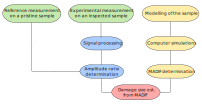
\includegraphics[width=0.95\textwidth]{flowchart.png}

			\caption{A flowchart representing the process for damage size estimation}

		\end{figure}

	\end{frame}

%%%%%%%%%%%%%%%%%%%%%%%%%%%%%%%%%%%%%%%%%%%%%%%%%%%%%%%%%%%%%%%%%%%%%%%%%%%%%%%%%%%%%%%%%%%%%%%%%%%%%%%%%%
\section{Development of the HSP model}

	\begin{frame}[label=frame6]{HSP sample configuration}

		\begin{table}

			\centering \footnotesize

			\caption{Geometry of HSP [mm]}

			%\begin{tabular}{@{}ccccccc@{}} % remove spaces from vertical lines

			\begin{tabular}{ccccccccccccc} 

				%\hline

				\toprule

				\multicolumn{3}{c}{\textbf{skin}} & {\textbf{adhesive}} & \multicolumn{6}{c}{\textbf{core}} & \multicolumn{2}{c}{\textbf{pzt}} & {\textbf{glue}}\\

				\multicolumn{3}{c}{CFRP $[0^\circ,90^\circ]_s$} & {EA3479B} & \multicolumn{6}{c}{aluminium} & \multicolumn{2}{c}{NCE51} & {CA}\\ 

				%	\hline \hline

				\cmidrule(lr){1-3} \cmidrule(lr){4-4} \cmidrule(lr){5-10} \cmidrule(lr){11-12} \cmidrule(lr){13-13}

				L & W & $g_s$ & $g_a$ & $h_1$ & $h_2$ & $l_1$ & $l_2$ & $g_c$ & $w_c$ & $\Phi$ & $g_t$ & $g_g$\\ 

				%\hline

				%\midrule

				\cmidrule(lr){1-3} \cmidrule(lr){4-4} \cmidrule(lr){5-10} \cmidrule(lr){11-12} \cmidrule(lr){13-13}

				500 & 500 & 1.5 & 0.05 & 11 & 5 & 10.4 & 6 & 14.5 & 0.1 & 10 & 0.5 & 0.05\\

				%\hline 

				\bottomrule 

			\end{tabular} 

			\label{tab:panel_geo}

		\end{table}

		\begin{figure}

			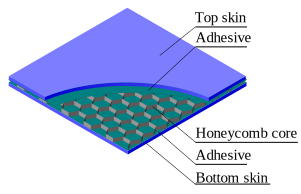
\includegraphics[width=1\textwidth]{honeycomb.png}

			\caption{(\textbf{a}) top view of HSP, (\textbf{b}) panel components, (\textbf{c}) details of the honeycomb cell}

		\end{figure}

	\end{frame}

	
\begin{frame}[label=frame7]{Basis of the Spectral Element Method}
	\begin{itemize}
		\item Division of the domain into non-overlapping finite element
		\item Nodes distribution - endpoints of the element and roots of the first derivative of Legendre polynomial \(\mathcal{P}\) of degree \(p\):
			\begin{equation*}
				(1-\xi^2)\mathcal{P}'_{p}(\xi)=0.
				\label{eq:nodes}
			\end{equation*}
		\item Gauss-Lobatto-Legrendre (GLL) integration scheme:
			\begin{equation*}
				{w(\xi)} = \frac{2}{p(p+1)(\mathcal{P}_{p}(\xi))^2}.
				\label{eq:weight}
			\end{equation*}
		\item Imposing external force $\textbf{f}_{ext}$ and boundary Condition
		\item Equation of motion:
		\begin{equation*}
			\label{eq:motion}
			\textbf{M} \ddot{d} + \textbf{D} \dot{d} + \textbf{K} d = f_{ext}
		\end{equation*}
		\item Diagonal mass matrix \(\textbf{M}\)
	\end{itemize}
\end{frame}

\begin{frame}[label=frame8]{The full core geometry model (FCGM)}

	\begin{columns}[T]

		\column{0.5\textwidth}

		\begin{block}{2D elements}

		\begin{itemize}

			\item core

			\item adhesive layer

		\end{itemize}

		\end{block}

		\column{0.5\textwidth}

		\begin{figure}

			\includegraphics[width=1\linewidth]{figs/2d_se}

			\caption{Two-dimensional spectral element}

			\label{fig:2dse}

		\end{figure}

	\end{columns}

	\begin{columns}[T]

		\column{0.5\textwidth}

		\begin{block}{3D elements}

			\begin{itemize}

				\item skin

				\item pzt

			\end{itemize}

		\end{block}

		\column{0.5\textwidth}

		\begin{figure}

			\centering

			\includegraphics[width=1\linewidth]{figs/3d_se}

			\caption{Three-dimensional spectral element}

			\label{fig:3dse}

		\end{figure}

	\end{columns}

\end{frame}

\begin{frame}[label=frame9]{Meshes for the components with the interfaces}

\begin{figure}

	\includegraphics[width=1\linewidth]{struct_mesh.png}

	\caption{The spectral elements with the nodes distribution for (\textbf{a}) the wall of the core, (\textbf{b}) the adhesive layer and the skin plate, (\textbf{c}) cyanoacrylate glue mesh with the second-order curve at the boundary and the PZT transducers.}

	\label{fig:elements}

\end{figure}

\end{frame}

	\begin{frame}[label=frame10]{Meshes for the components with the interfaces}

		\begin{figure}

			\includegraphics[width=1\linewidth]{panel_mesh.png}

			\caption{The meshes of HSP components and the interfaces}

			\label{fig:panel_mesh}

		\end{figure}

	\end{frame}

	\begin{frame}[label=frame11]{Disbonds models}

		\begin{figure}

			\includegraphics[width=1\linewidth]{disbond.png}

			\caption{The damaged area in the: (\textbf{a}) experimental sample, (\textbf{b}) numerical model with removed cells and (\textbf{c}) numerical model with interface decoupling}

			\label{fig:disbonds}

		\end{figure}

	\end{frame}

\begin{frame}[label=frame11]{Comparison of the models - healthy state}

	\begin{figure}

		\includegraphics[width=0.9\linewidth]{models_comparison_0.png}

		
	\end{figure}

\end{frame}
\begin{frame}[label=frame11]{Comparison of the models - damage 90 mm}

	\begin{figure}

		\includegraphics[width=0.9\linewidth]{models_comparison_90.png}
	\end{figure}

\end{frame}

%%%%%%%%%%%%%%%%%%%%%%%%%%%%%%%%%%%%%%%%%%%%%%%%%%%%%%%%%%%%%%%%%%%%%%%%%%%%%%%%%%%%%%%%%%%%%%%%%%%%%%%%%
	\section{Experimental Validation of the Method }

	\begin{frame}[label=frame12]{Experimental validation setup}

		\begin{columns}[T]

			\column{0.5\textwidth}

			\begin{figure}

				\includegraphics[width=0.8\linewidth]{pzt_setup.png}

				\caption{The PZT setup, (\textbf{a}) the wave generation/acquisition	instruments: DMU - the data management unit, G1, G2 - the arbitrary wave generator, O - the oscilloscope, HVA - the voltage amplifier, LWDS - the Lamb Wave Detection Systems, (\textbf{b}) the specimen with the PZTs}

				\label{fig:pzt_setup}

			\end{figure}

			\column{0.5\textwidth}

			\begin{figure}

				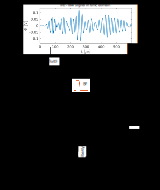
\includegraphics[width=1\linewidth]{signal_processing.png}

				\caption{Flowchart for signal processing}			\label{fig:signal_processing}

			\end{figure}

		\end{columns}

		
	\end{frame}

	\begin{frame}[label=frame13]{Experimental validation results}

		\begin{columns}[T]

			\column{0.5\textwidth}

			\begin{figure}

				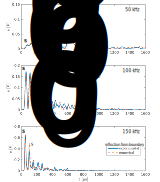
\includegraphics[width=1\linewidth]{single_skin.png}

				\caption{Signals for \textbf{single CFRP skin}}

				\label{fig:single_skin}

			\end{figure}

			\column{0.5\textwidth}

			\begin{figure}

				\includegraphics[width=1\linewidth]{HSP_full.png}

				\caption{Signals for \textbf{HSP} based on the full core geometry model (\textbf{FCGM})}

				\label{fig:HSP_full}

			\end{figure}

		\end{columns}

	\end{frame}

	\begin{frame}[label=frame14]{Experimental validation results - single CFRP}

		\begin{table}

			\centering

			\caption{\label{tab:group_velocity_cfrp} Comparison between amplitudes and group velocities  obtained and experiments for HSP}
			\begin{tabular}{cccccccc}

				\toprule

				& & \multicolumn{3}{c}{\(C_g\)} & \multicolumn{3}{c}{Amp.}\\

				Mode & Frequency & Exp. & Num. & \(\delta\)& Exp. & Num. & \(\delta\)\\

				& kHz & m/s & m/s & \% & mV & mV & \% \\

				\midrule

				\multirow{3}{*}{$S_0$} & 50 & 6079 & 5865 & \textcolor{green}{3.52}& 12 & 171 & \textcolor{red}{25.0} \\

				&100& 5571 & 5747 & \textcolor{green}{3.16} & 115 & 162 & \textcolor{green}{5.26}\\

				&150& 5764 & 5698 & \textcolor{green}{1.15} & 648 & 664 & \textcolor{green}{2.47}\\

				\midrule

				\multirow{3}{*}{$A_0$} &50& 1341 & 1325 & \textcolor{green}{0.74} & 134 & 125 & \textcolor{green}{6.72}\\

				&100& 1550 & 1396 & \textcolor{green}{9.74} & 84 & 104 & \textcolor{red}{23.8}\\
				\bottomrule

			\end{tabular}

		\end{table}

	\end{frame}

	\begin{frame}[label=frame14]{Experimental validation results - HSP}

		\begin{table}

			\centering

			\caption{\label{tab:group_velocity_hsp} Comparison between amplitudes and group velocities obtained from the simulations based on the FCGM and experiments for HSP}

			\begin{tabular}{cccccccc}

				\toprule

				& & \multicolumn{3}{c}{\(C_g\)} & \multicolumn{3}{c}{Amp.}\\

				Mode & Freq. & Exp. & FCGM & \(\delta\) & Exp. & FCGM & \(\delta\)\\

				& kHz & m/s & m/s & \% & mV & mV & \%\\

				\midrule

				\multirow{3}{*}{$S_0$} & 50 & 6452 & 8696 & {34.78}& 32 & 6 & \textcolor{red}{81.25}\\

				&100& 5263 & 5128 & \textcolor{green}{2.57}& 369 & 314 & \textcolor{green}{14.91}\\

				&150& 5085 & 5217 & \textcolor{green}{2.60}& 1341 & 1239 & \textcolor{green}{7.61}\\

				\midrule

				\multirow{2}{*}{$A_0$} & 50 & 966 & 926 & \textcolor{green}{4.14} & 1316& 76 & {22.58}\\

				& 100 & 2174 & 2151 & \textcolor{green}{1.06} & 137 & 179 & {30.66}\\

				\bottomrule

			\end{tabular}

		\end{table}

	\end{frame}

	\section{Model-Assisted Damage Identification Function}

	%%%%%%%%%%%%%%%%%%%%%%%%%%%%%%%%%%%%%%%%%%%%%%%%%%

	\begin{frame}[label=frame]{Model-Assisted Damage Identification Function (MADIF)}

		\begin{figure}

			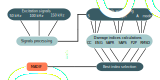
\includegraphics[width=0.9\linewidth]{madif_extract.png}
		\end{figure}

	\end{frame}

	\section{Conclusions}

	%%%%%%%%%%%%%%%%%%%%%%%%%%%%%%%%%%%%%%%%%%%%%%%%%%

	\begin{frame}[label=frame]{Conclusions}

		
	\end{frame}

\end{document}